%% Creator: Inkscape inkscape 0.48pre0, www.inkscape.org
%% PDF/EPS/PS + LaTeX output extension by Johan Engelen, 2010
%% Accompanies image file 'wave_mesh' (pdf, eps, ps)
%%
%% To include the image in your LaTeX document, write
%%   \input{<filename>.tex}
%%  instead of
%%   \includegraphics{<filename>.pdf}
%% To scale the image, write
%%   \def{\svgwidth}{<desired width>}
%%   \input{<filename>.tex}
%%  instead of
%%   \includegraphics[width=<desired width>]{<filename>.pdf}

\begingroup
  \makeatletter
  \providecommand\color[2][]{%
    \errmessage{(Inkscape) Color is used for the text in Inkscape, but the package 'color.sty' is not loaded}
    \renewcommand\color[2][]{}%
  }
  \providecommand\transparent[1]{%
    \errmessage{(Inkscape) Transparency is used (non-zero) for the text in Inkscape, but the package 'transparent.sty' is not loaded}
    \renewcommand\transparent[1]{}%
  }
  \providecommand\rotatebox[2]{#2}
  \ifx\svgwidth\undefined
    \setlength{\unitlength}{414.221875pt}
  \else
    \setlength{\unitlength}{\svgwidth}
  \fi
  \global\let\svgwidth\undefined
  \makeatother
  \begin{picture}(1,0.46220851)%
    \put(0,0){\includegraphics[width=\unitlength]{pics/wave_mesh.ps}}%
    \put(-0.01,0.43937051){\color[rgb]{0,0,0}\makebox(0,0)[lb]{\smash{$k_\perp$}}}%
    \put(0.93459121,0.00482079){\color[rgb]{0,0,0}\makebox(0,0)[lb]{\smash{$k_\parallel$}}}%
    \put(-0.00,0.15932735){\color[rgb]{0,0,0}\makebox(0,0)[lb]{\smash{$k_l$}}}%
    \put(-0.005,0.30417726){\color[rgb]{0,0,0}\makebox(0,0)[lb]{\smash{$k_u$}}}%
    \put(0.03652179,0.02413411){\color[rgb]{0,0,0}\makebox(0,0)[lb]{\smash{$0$}}}%
     \put(0.08480509,0.12070071){\color[rgb]{0,0,0}\makebox(0,0)[lb]{\smash{$\vartheta$}}}%
  \end{picture}%
\endgroup
